% Crucial Preamble
\documentclass[12pt,letterpaper]{article} \usepackage{amsmath} \usepackage{graphicx} \usepackage[margin=1in]{geometry} \usepackage{longtable}  \usepackage{amssymb}

% Extra Preamble
\usepackage{fancyhdr} \usepackage{enumitem} \usepackage{float} \usepackage{soul}
\usepackage{multicol} \usepackage[compact]{titlesec} \usepackage{listings}


% frames with display breaks
\usepackage{mdframed}
\allowdisplaybreaks

% change spacing
\usepackage{setspace}
\setlength{\parskip}{0.4\baselineskip}

% Remove paragraph indentation
\setlength{\parindent}{0pt}

% Reduce space before and after section headings
%\titlespacing*{\section}{0pt}{0.1\baselineskip}{0.2\baselineskip}

% changes font
%\renewcommand{\familydefault}{\sfdefault}

% adds header and footer
\pagestyle{fancy}
\fancyhead{} \fancyhead[C]{ADM 1100 Cheat Sheet} \fancyhead[L]{ADM1100} \fancyhead[R]{Owen Daigle}
\fancyfoot{} \fancyfoot[C]{\thepage}


\begin{document}
	
	\begin{center}
		\Large\textbf{ADM 1100 Cheat Sheet} \\
		\vspace{0.5em}
	\end{center}
	
		We are going in a non chronilogical order with the chapters for this course, so the cheat sheet will be in a non chronilogical order as well.
		
		This course is a lot about memorization :-(. 
		
		\section{Chapter 4: Starting a Business}
		
		\subsection{Important Definitions}
		A \textbf{Small Business} is an \textit{owner managed business} with fewer than 100 employees. 
		
		A \textbf{New Venture} is a business opened in the \textit{last 12 months}.
		
		\textbf{Entrepreneurship} is the process of identifying and capitalizing on a marketplace opportunity. 
		
		An \textbf{Entrepreneur} is someone who recognises and seizes oppurtunites. 
		
		An \textbf{Intrapreneur} is someone who creates something new within an existing larg  organization. 
		
		\subsection{Business Plan}
		
		A \textbf{business plan} has the following parts:
		\begin{enumerate}[]\item Cover Page \item Executive Summary (Short overview of the plan)\item Table of Contents\item Company Description (Type, form, of company primary product of company, etc.)\item Product or Serivce Decription (and what is unique about it)\item Marketing (Market Analysis and Plan)\item Operating Plan (Where to get Labour, Raw materials, facilities, etc.)\item Management (Who are they)\item Financial Plan \item Appendix (Extras)\end{enumerate}
		
		\subsection{Alternative Ways of Getting a Business}
		
		\subsubsection{Buying an Existing Business}
		This has \textbf{pros} such as established clients, finances, employees, line of supply, and it is less risky. 
		
		It has \textbf{con} such as being stuck with legacy decision making, financial health, and reputation.
		
		So basically it depends on what the previous owners did to the reputation, could be a good reputation or bad one. 
		
		\subsubsection{Taking over a Family Members Business}
		This can have problems such as who takes over the business, how much it should cost, should other family members automatically get a job, etc. 
		
		\subsubsection{Buying a Franchise}
		This has \textbf{pros} such as expert advice, training provided, low failure rates, and all reputation and stuff is already existing. 
		
		\subsection{Forms of Businesses}
		\begin{center}
			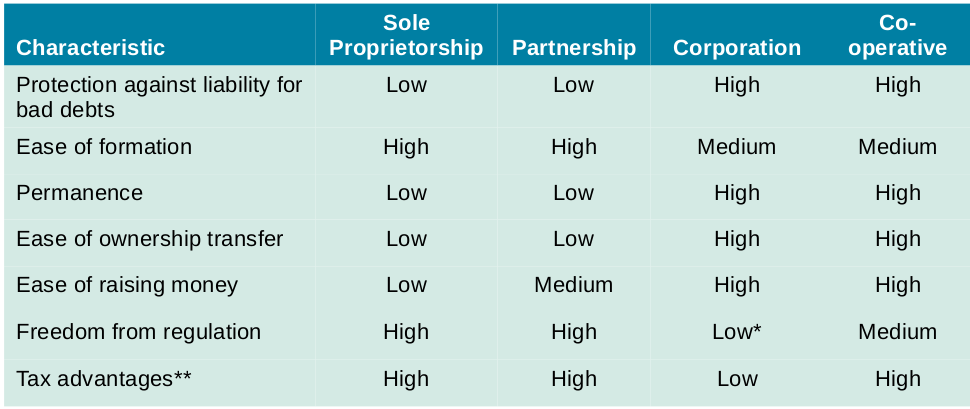
\includegraphics[width=0.7\linewidth]{screenshot001}
		\end{center}
		
		\subsubsection{Sole Proprietorship}
		This basically means that you are in charge of everything. You get to pay minimum fees, do stuff how you want, but if it goes wrong, it is all on you. 
		
		\subsubsection{Partnerships}
		This is when multiple people pool together to share resources, and sometimes liability.
		
		If someone is a \textbf{general partner}, then they share the liability with the other general partners. 
		
		If someone is a \textbf{limited partner}, then they are \textbf{not involved in day to day activities} and do not have any liability.
		
		\subsubsection{Corporation}
		These are \textbf{seperate entities} from the owner. 
		
		If it is \textbf{public}, then anyone can buy shares of the company.
		
		If it is \textbf{private}, then only some people can buy the shares of the company. 
		
		These have limited liabilities for the employees, and professional management, but they have start up costs, and lots of taxation and regulations. 
		
		\subsubsection{Cooperatives}
		These are organiazations created between \textbf{multiple owners} to share supplies. 
		
		They have \textbf{limited liability} for the members, equal voting for all of the members, and there are not many tax problems. 
		
		\section{Chapter 15: Managing Financing}
		\subsection{Short Term Funds}
		Businesses need short term (\textbf{operating}) funds for raw materials, wages, power, rent. 
		
		These can be obtained through trade credit (granting credit to another firm), secured loans (loan with collateral), unsecured loans (loan without collateral) or factoring accounts receivable. 
		
		\subsection{Long Term Funds}
		They also need long term (\textbf{capital}) funds for land, machinery, etc. 
		
		These can be obtained from debt financing (long term loans, or bonds), equity financing (stocks), or hybrid financing (preffered shares are stocks that have no voting rights). 
		
		\subsection{Financial Manager}
		This is a person whose rule is overseeing cash flow management, financial planning, nad financial control.
		
		They obtain funds, manage risk, and conduct the day to day financial activities. 
		
		\subsubsection{Cash Flow Management}
		This is managing the times when the cash is flowing in at a fast rate, and when it is flowing out (not much business).
		
		\subsubsection{Financial Control}
		This is checking the \textbf{performance against plans. }
		
		This is also creating \textbf{budgets} so we don't run out of cash. 
		
		\subsubsection{Financial Planning}
		This is a plan to achieve a desired financial status. 
		
		\subsection{Risk Management}
		Lower risk conserves the firms financial power by minimizing the financial effect of negative events. 
		
		
		\section{Chapter 11: Accounting}
		\textbf{Financial Accounting} keeps external parties informed about the finances. 
		
		\textbf{Managerial Accounting} keeps managers informed about the finances so they can plan.
			
		\subsection{Accounting Equation}
		This equation is: 
		\begin{align*}
			\text{Assets} = \text{Liabilities} + \text{Owners' Equity}
		\end{align*}
		where the assets are anything of economic value, liabilities are any debts, and the owner's equity is any positive difference between the firms assets and liabilities. 
		
		\subsection{Financial Statements}
		
		\subsubsection{Balance Sheets}
		This shows detailed information about \textbf{assets, liabilities, and the owners equity. }
		
		It is a \textbf{snapshot} at a point in time. 
		
		For the assets part of this, we have:
		
		\textbf{Current Assets }are stuff like Cash, Accounts receivable (bills needed to be paid by customers), inventory (unsold merchandise), and prepaid expenses (office supplies, and paid bills such as rent).
		
		\textbf{Fixed assets }have a \textbf{long term value }such as land, buildings, machinery, etc. 
		
		\textbf{Intangible assets }are not physical, but they have a value such as patents, and trademarks. 
		
		\textbf{Goodwill} is also an asset. 
		
		For the liabilities, we have:
		
		\textbf{Current Liabilities} are debts that must be repaid \textbf{within one year.}
		
		\textbf{Long Term liabilities} are debts needed to be repaid in more than one year. 
		
		There is also the \textbf{Owner's Equity} which is the owners holdings in the firm. 
 		\subsubsection{Income Statements}
 		This is the profit and loss statement over a period. 
 		
 		All revnues and expenses are listed including depreciation (value of a building decreases with normal wear and tear).
		
		\subsubsection{Statements of Cash Flow}
		This shows the ccash in, and the cash out from operations, investments, and financing activities. 
		
		\subsection{Financial Ratios}
		There are 3 types of ratios:
		
		Solvency Ratios are the ability to meet total debt obgligations. 
		
		Activity Ratios measure the efficiency in different ways. 
		
		Profitability Ratios measure how well the sales can sustain the business. 
	
\end{document}